\section{Entscheidungsbäume, Boosting und Bagging}
\label{mainsec:trees}
\textit{Annalena Gutheil, Matthias Volland}

Die Verwendung von baumartigen Strukturen zur Klassifikation von Daten bietet sich aus mehreren Gründen an. 
%Einerseits handelt es sich bei Bäumen um eine Datenstruktur, die häufig in der Informatik verwendet wird und daher vom Verständnis intuitiver ist, als beispielsweise ein neuronales Netzwerk oder eine SVM. 
Einerseits handelt es sich bei Bäumen um eine Datenstruktur, die häufig in der Informatik verwendet wird. Durch ihre nachvollziehbare hierarchische Struktur, sind sie vom Verständnis intuitiver als beispielsweise eine neuronales Netz.
Andererseits ist das Erzeugen von Bäumen im Allgemeinen relativ effizient, was bei Machine-Learning-Algorithmen 
in der Traningsphase wichtig ist. Das Verwenden bzw. Durchlaufen eines Baumes hat lediglich eine logarithmische Komplexität, 
so dass auch die Klassifikation durch einem Baum sehr effizient ist, sofern dieser nicht entartet ist~\cite{Marsland}. 

\subsection{Entscheidungsbäume}

Bäume zur Klassifikation von Daten werden auch als Entscheidungsbäume bezeichnet und bestehen aus Knoten, Kanten und Blättern. Knoten entsprechen dabei Merkmalen bzw. \glqq Features\grqq\ der zu klassifizierenden Daten und die Kanten an einem Knoten den verschiedenen Merkmalsausprägungen. 
Ein Knoten kann entweder einen weiteren Knoten als Kind haben (also ein weiteres Merkmal) oder aber ein Blatt, was einer Klasse entspricht.

\subsubsection{Einführendes Beispiel}
Um beispielsweise verschiedene Gemüsesorten zu klassifizieren, könnten im einfachsten Fall Farbe und Form als Unterscheidungsmerkmale dienen. Wenn jedes Objekt der Testmenge die Merkmale (Form, Farbe) hat, würde eine Tomate mit (rund, rot) beschrieben, eine Gurke mit (länglich, grün) und eine Möhre mit (länglich, orange).

Ein Entscheidungsbaum zur Klassifikation könnte dann aus einem Wurzel-Knoten bestehen, der zunächst anhand der Form 
des zu klassifizierenden Objektes eine erste Entscheidung vornimmt. Als zweites Entscheidungskriterium bliebe dann die Farbe des Objektes. In Abbildung~\ref{fig:tree} ist der resultierende Entscheidungsbaum abgebildet. Zur Unterscheidung, ob es sich bei dem Objekt um eine Tomate handelt, wird in dem Beispiel ausschließlich die Information über die Form benötigt. Um Gurke und Tomate zu unterscheiden, muss in der nächsten Ebene noch die Farbe des Objekts geprüft werden.

%Da eine Tomate rund ist und Gurken und Möhren länglich, 
%hätte der Wurzelknoten zur Unterscheidung der Form die beiden Kanten \glqq rund\grqq\ und \glqq länglich\grqq\ . Da in dem Beispiel nur Tomaten rund sind, hätte die Kante mit dem Attribut \glqq rund\grqq\ das Blatt bzw. die Klasse \glqq Tomate\grqq\ als Kind. Gurken und Möhren haben 
%jedoch beide eine längliche Form, so dass diese nicht alleine aufgrund der Form unterschieden werden können. Daher müsste die 
%Kante mit dem Merkmal \glqq länglich\grqq\ in einen weiteren Knoten münden, durch welchen die Testmenge in einem nächsten Schritt anhand der Farbe weiter unterteilt werden müsste. Dieser Entscheidungsknoten hätte die Kanten \glqq rot\grqq , \glqq grün\grqq\ und \glqq orange\grqq, die jeweils in einem Blattknoten mit den Klassen \glqq Tomate\grqq , \glqq Gurke\grqq\ und \glqq Möhre\grqq\ müden würden.

% Set the overall layout of the tree
\tikzstyle{level 1}=[level distance=3.5cm, sibling distance=3.5cm]
\tikzstyle{level 2}=[level distance=3.5cm, sibling distance=2cm]

% Define styles for bags and leafs
\tikzstyle{bag} = [text width=4em, text centered]
\tikzstyle{end} = [circle, minimum width=3pt,fill, inner sep=0pt]

% The sloped option gives rotated edge labels. Personally
% I find sloped labels a bit difficult to read. Remove the sloped options
% to get horizontal labels. 
\begin{figure}[htbp] \centering
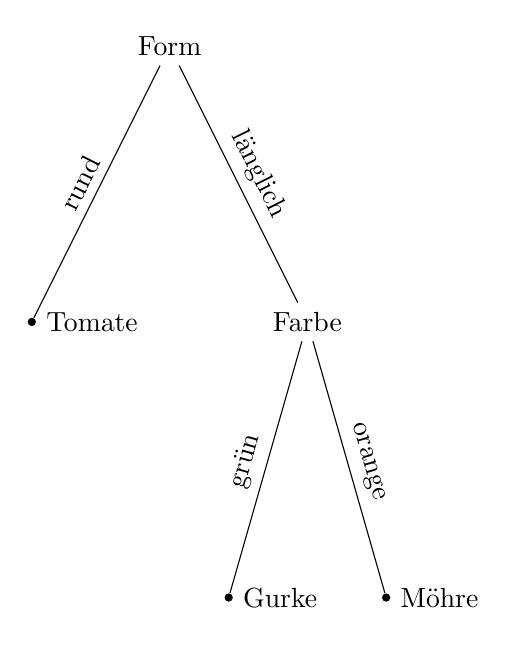
\begin{tikzpicture}[sloped]
\node[bag] {Form}
    child {
        node[end, label=right: {Tomate}]{}        
            edge from parent 
            node[above] {rund}
    }
    child {
        node[bag] {Farbe}        
            child {
                node[end, label=right:
                    {Gurke}] {}
                edge from parent
                node[above] {grün}
            }
            child {
                node[end, label=right:
                    {Möhre}] {}
                edge from parent
                node[above] {orange}
            }
            edge from parent 
            node[above] {länglich}
    }
    ;
\end{tikzpicture}
\caption{Entscheidungsbaum}
\label{fig:tree}
\end{figure}

In dem Beispiel hätte als erstes Unterscheidungsmerkmal auch die Farbe dienen können, wodurch direkt in einem Schritt alle drei Gemüsesorten hätten klassifiziert werden können. Somit hat die Wahl der Reihenfolge der Merkmale einen wesentlichen Einfluss auf die Form des Entscheidungsbaumes sowie die Effizienz, mit der Testdaten klassifiziert werden können. Weiterhin können durch die ungünstige Wahl von Kriterien verschiedene Klassen mehrfach in dem Entscheidungsbaum vorkommen, was darauf schließen lässt, dass der Baum aufgrund der Redundanz mehr Knoten enthält, als für eine Klassifizierung notwendig wäre.

\subsubsection{Entscheidungskriterien}
Maße für die Güte eines Baumes können beispielsweise die Baumhöhe, die Anzahl der Blätter sein oder die Summe aller Pfade, was auch als externe Pfadlänge bezeichnet wird. Das Problem zu entscheiden, ob ein Entscheidungsbaum mit einer maximalen externen Pfadlänge existiert, ist NP-vollständig. Es gibt jedoch verschiedene Kriterien, nach denen die Reihenfolge der Merkmale so gewählt werden kann, dass ein möglichst kompakter und damit effizienter Entscheidungsbaum entsteht. Ein Ansatz für das Erstellen eines möglichst guten Entscheidungsbaumes besteht darin zu berechnen, wie groß der Informationsgehalt der zu unterscheidenden Merkmale ist~\cite{Shannon}. Der Informationsgehalt eines Merkmals bestimmt sich daraus, wie häufig es vorkommt und ist definiert als 
\[I = -log \left( p_i \right)\] wobei $p_i$ die relative Häufigkeit ist, mit der das Merkmal $i$ vorkommt. Ein sehr häufig vorkommendes Merkmal hat dementsprechend einen niedrigeren Informationsgehalt als ein seltenes Merkmal. Der Mittlere Informationsgehalt aller Merkmale wird auch als Entropie bezeichnet lässt sich dann mit Hilfe der Formel 
\[E = - \sum \limits_{i=1}^n p_i \cdot \log \left( p_i \right)\] berechnen, wobei $n$ die Menge aller Merkmale ist und $p_i$ die relative Häufigkeit des Merkmals $i$.
Um nun das Vorkommen der Merkmale in Relation zu den möglichen Klassifikationen zu setzen, wird die bedingte Wahrscheinlichkeit für die Merkmale bezogen auf die möglichen Klassen ermittelt, woraus sich der mittlere Informationsgewinn ermitteln lässt. Dieser ist definiert als 
\[H = - \sum \limits_{i=1}^n p_i \cdot \left( \sum \limits_{j=1}^m \frac{x_{ij}}{x_i} \cdot \log \left(\frac{x_{ij}}{x_i}\right)\right) \] wobei $n$ die Anzahl der Merkmale ist und $m$ die Anzahl der Klassen. Der Wert $x_i$ beschreibt die Anzahl der Vorkommen der Merkmalsausprägung $i$ und $x_{ij}$ die Anzahl der Vorkommen dieser Merkmalsausprägung unter der Bedingung, dass das Objekt zur Klasse $j$ gehört.
Beim Erstellen eines Entscheidungsbaumes ist dann das Merkmal für die Teilung der Datenmenge in Teilbäume auf der aktuellen Ebene am interessantesten, was den größten mittleren Informationsgewinn \textit{H} hat, also die innere Summe minimal ist.
Da sich durch das Merkmal \glqq Farbe\grqq\ aus dem vorigen Beispiel direkt alle möglichen Klassen unterscheiden lassen, hat dieses Merkmal z.B. einen höheren Informationsgewinn als das Merkmal \glqq Form\grqq\ und bietet sich daher als erstes Entscheidungskriterium an.

Ein anderes Maß zur Auswahl von geeigneten Entscheidungsmerkmalen ist die sogenannte \glqq Reinheit\grqq\ von Merkmalen~\cite{Gini}. Die Reinheit eines Merkmales ergibt sich daraus, wie viele verschiedene Klassen die jeweiligen Merkmalsausprägungen beinhalten. Das Attribut \glqq Farbe\grqq\ aus dem vorigen Beispiel führt zu drei Blattknoten, bei denen durch jeden Knoten genau eine Klasse repräsentiert wird (nämlich jeweils die Klassen Tomate, Gurke und Möhre) während beim Merkmal \glqq Form\grqq\ sowohl Möhren als auch Gurken als mögliches Ergebnis in Frage kommen, falls das zu klassifizierende Objekt die Merkmalsausprägung \glqq länglich\grqq\ hat. Die Reinheit ist dementsprechend ein Maß dafür, wie groß das Risiko einer falschen Klassifikation ist. Ziel ist es anhand von Merkmalen Teilungen im Entscheidungsbaum vorzunehmen, die ein möglichst geringes Risiko für falsche Klassifikationen haben.

%Entscheidungsbäume funktionieren nach dem \glqq teile und herrsche\grqq\ -Prinzip. 
%Beginnend beim Wurzelknoten wird bei jedem Knoten mithilfe einer Testfunktion berechnet, welche Abzweigung genommen werden muss. 
%Ist man am Blattknoten angekommen, ist dies die zur Eingabe gehörende Klasse~\cite{alpaydin:maschinelles_lernen, borgelt:data_mining}.

\subsection{Ensemble Learning}
Die Idee von Ensemble Learning ist es, mehrere Klassifikatoren gleichzeitig zu verwenden anstatt eines einzigen Klassifikators, um bessere Ergebnisse zu erzielen~\cite{Opitz99popularensemble}. Der Vorteil bei der Verwendung mehrerer Klassifikatoren ist es, dass nicht ein einzelner Klassifikator alle Klassen möglichst gut unterscheiden können muss, sondern dass mehrere (unabhängig voneinander gesehen schwächere) Klassifikatoren zusammen einen starken Klassifikator bilden können. Wichtig ist dabei lediglich, dass jeder der schwachen Klassifikatoren geringfügig besser sein muss als raten, also bei einer binären Klassifikation eine Erfolgsrate von mehr als 50\% hat.
Bezugnehmend auf das einführende Beispiel zur Klassifikation verschiedener Gemüsesorten könnte man also beispielsweise einen Klassifikator verwenden, der sehr gut anhand der Form klassifizieren kann und einen weiteren anhand der Farbe. Ein Nachteil von Ensemble Learning ist jedoch, dass der Trainingsaufwand mit der Anzahl der Klassifikatoren steigt. Da bei Entscheidungsbäumen das Training verglichen mit anderen Klassifikatoren jedoch relativ effizient ist, bieten sich Entscheidungsbäume besonders als Klassifikatoren für Ensemble Learning an. Im Folgenden werden daher zwei verschiedene Ansätze des Ensemble Learning vorgestellt.


\subsubsection{Bagging}
Eine einfache Methode, um mehrere Klassifikatoren miteinander zu kombinieren, wird als Bagging bezeichnet, eine Abkürzung für Bootstrap Aggregating~\cite{Breiman96baggingpredictors}. Der Name steht im Zusammenhang mit der Ziehung von Stichproben aus einer Menge, wo ein \glqq bootstrap sample\grqq\ eine Bezeichnung dafür ist, ein Testdatensatz \glqq mit Zurücklegen\grqq\ aus der Testmenge zu ziehen. Somit können manche Testdaten mehrfach, andere gar nicht in der Trainingsmenge vorhanden sein. Durch die daraus resultierenden unterschiedlichen Trainingsdaten entstehen Klassifikatoren, die verschiedene Klassen unterschiedlich gut unterscheiden können. Die Klassifikation erfolgt dann aufgrund einer Mehrheitsentscheidung.

\subsubsection{Boosting}
Boosting unterscheidet sich zu Bagging dahingehend, dass während des Trainings immer mit den gleichen Trainings- und Testdaten gearbeitet wird und nicht eine zufällige Auswahl verwendet wird.
Das bekannteste Boosting-Verfahren heißt AdaBoost und existiert seit Mitte der 90er Jahre~\cite{Freund95adecision-theoretic}. Die grundsätzliche Idee bei dem Verfahren ist es, jeden Datensatz um ein zusätzliches Gewicht als Maß dafür zu erweitern, wie fehlerbehaftet dieser Datensatz in den vorigen Trainingsrunden klassifiziert worden ist. Durch dieses Gewicht, welches im Laufe der Klassifikation immer wieder angepasst wird, werden falsch klassifizierte Daten hervorgehoben und stärker fokussiert. AdaBoost ist ein iterativer Algorithmus, der für jede neue Iteration die Fehlklassifikationen des vorherigen Trainings mit einbezieht mit dem Ziel, im besten Fall am Ende alle Testdaten richtig zuzuordnen. Das Gewicht berechnet sich anhand des jeweiligen Fehlers $\epsilon$, der sich aus der Summe der Gewichte der falsch klassifizierten Datenpunkte zusammensetzt. Das Gewicht dieser Datenpunkte wird mit
$ \alpha = \frac{\epsilon}{(1-\epsilon)} $ 
multipliziert, sodass die \glqq schwierig\grqq\ zu klassifizierenden Daten stärker berücksichtigt werden. Ziel ist es mit jedem weiteren Training einen neuen Klassifikator zu erhalten, der ein niedrigeren Fehler hat als in den vorangegangenen Iterationen. Die Trainingsphase kann dadurch beendet werden, dass eine feste Anzahl an auszuführenden Iterationen vorgegeben wird oder wenn das Optimum, dass alle Datenpunkte richtig klassifiziert wurden, erreicht wurde.

\subsection{Datenaufbereitung}
\label{sect:Trees_Datenaufbereitung}

Die zu klassifizierenden Gesten unterscheiden sich dahingehend, dass sie die Bandbreite 
des Frequenzspektrums um den Referenzton in unterschiedlicher Weise verschieben bzw. vergrößern. 
Um eine Geste zu erkennen, werden daher die Amplituden der aufgezeichneten Frequenzen 
um die Amplitude der Frequenz des Referenztons im Spektrum in beiden Richtungen analysiert. 
Relevant für die Erkennung der Gesten sind dabei im Allgemeinen nur diejenigen Frequenzanteile 
um den Referenzton, deren Amplitude den Grenzwert von 10\% der Amplitude des Referenztones nicht unterschreitet. 
In Ausnahmefällen können die Frequenzanteile einer Geste im Spektrum durch ein lokales Minimum vom Referenzton 
separiert sein. Daher wird zusätzlich nach einem weiteren Ausschlag im Spektrum gesucht, 
dessen Maximum mindestens 30\% der Amplitude des Referenztons entsprechen muss.


Eine Geste setzt sich zunächst aus 32 Einzelaufnahmen (Samples) zusammen, welche jeweils 
64 Amplitudenwerte beinhalten. Somit besteht eine Geste zunächst aus insgesamt 2048 Werten.
Da wie einführend beschrieben die Amplituden der Frequenzanteile einer Geste durch ein lokales Minimum vom Referenzton 
getrennt sein können, werden die Amplituden der einzelnen Samples zunächst mit einem Gauß-Filter geglättet, 
so dass Schwankungen aus dem Signal entfernt werden. 
Abbildung~\ref{fig:gauss} zeigt die Amplituden des Frequenzspektrums von einem Sample 
vor dem Glätten mit einem Gauß-Filter (rot) und danach (blau).

\begin{figure}[htbp] \centering
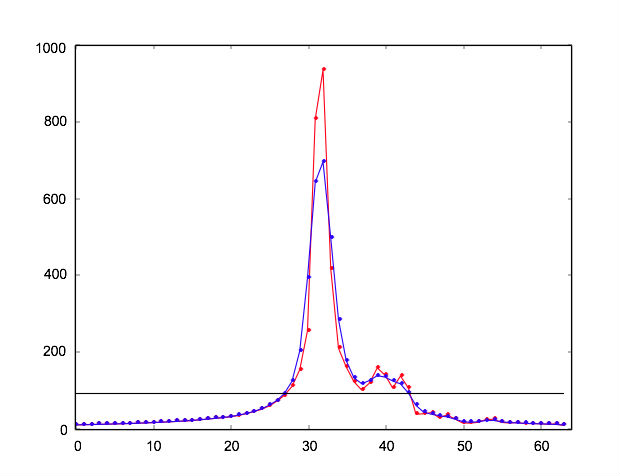
\includegraphics[height=60mm]{trees/gesture4-gauss1.jpg}
\caption{Rot: Ungefilterte Amplitudenwerte, Blau: Durch Gauß-Filter geglättete Amplitudenwerte}
\label{fig:gauss}
\end{figure}

Für die effiziente und robuste Klassifizierung der Gesten bietet es sich weiterhin an, 
die Komplexität der generierten Eingabedaten zu reduzieren. Dazu wird in jedem Sample einer Geste 
auf der linken und rechten Seite des Referenztons die Anzahl der Amplituden des geglätteten Signals ermittelt, 
deren Wert größer als 10\% ist. Der daraus resultierende Graph zeigt dann für eine Geste die zeitliche 
Änderung der Amplitudenanteile um den Referenzton auf der linken und rechten Seite an. Dieser Graph ist in Abbildung~\ref{fig:sum_of_bins} dargestellt, wobei die Anzahl der zum Referenzton gehörenden Amplituden aller Frequenzen unterhalb des
Referenztons in rot dargestellt sind, die Frequenzanteile oberhalb des Referenztons in blau.

\begin{figure}[htbp] \centering
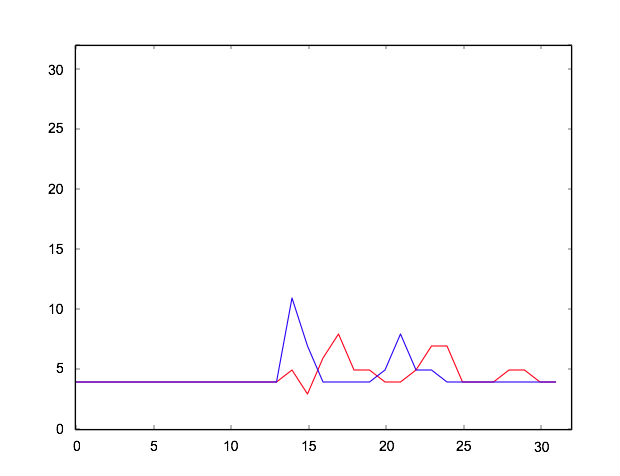
\includegraphics[height=60mm]{trees/gesture4-peaksize.jpg}
\caption{Frequenzanteile links (rot) und rechts (blau) von dem Referenzton}
\label{fig:sum_of_bins}
\end{figure}

Bei der in der Grafik dargestellten Geste handelt es sich um einen \glqq Double-Push\grqq , also eine Geste, bei der die Hand zweimal 
hintereinander schnell auf den Monitor bzw. das Mikrofon zubewegt wird. Diese Geste äußert sich in jeweils zwei aufeinander folgenden 
Verschiebungen der Frequenzen nach rechts (auf den Monitor zu bewegen) und links (vom Monitor weg bewegen). 
Diese Charakteristik lässt sich in der Grafik erkennen, da die Anzahl der zum Referenzton gehörenden Frequenzanteile zunächst nach rechts (erster Peak blau) und dann nach links (zweiter Peak rot) ansteigt. Aufgrund des \glqq \acl{DPO}\grqq\ erfolgt diese 
Verschiebung zweimal hintereinander, so dass insgesamt vier Ausschläge (zwei nach rechts und zwei nach links) zu erkennen sind. 
Somit kann in einem Schritt die Anzahl der Daten pro zu klassifizierender Geste von 32$\cdot$64=2048 Amplitudenwerten 
auf 2$\cdot$32=64 reduziert werden, wobei diese Werte keinen Rückschluss auf die genauen Frequenzanteile zulassen sondern 
ein Maß dafür sind, wie sich die Frequenzanteile ober- und unterhalb des Referenztons verändern.

Die daraus entstehenden Daten können in einem weiteren Schritt geglättet werden, da nur Amplitudenschwankungen ab einer gewissen 
Größe auf eine ausgeführte Bewegung schließen lassen. Dazu werden alle Schwankungen auf der rechten oder linken Seite entfernt, 
die unterhalb eines definierten Grenzwertes liegen. 
Abbildung~\ref{fig:filtered} zeigt ein gefilterten Graph, in dem alle Ausschläge entfernt werden, die kleiner als 2 sind:

\begin{figure}[htbp] \centering
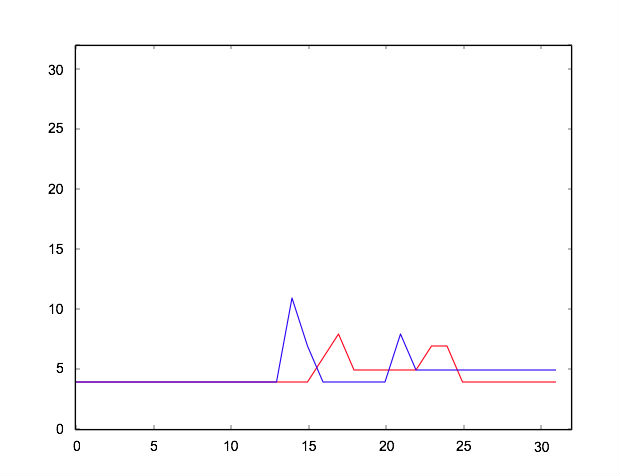
\includegraphics[height=60mm]{trees/gesture4-peaksize-smoothed.jpg}
\caption{Geglättete Frequenzanteile}
\label{fig:filtered}
\end{figure}

In einen dritten Schritt werden die Amplitudenwechsel dahingehend weiter geglättet, indem zunächst die Anzahl der am häufigsten 
auftretenden Frequenzanteile auf der linken und rechten Seite vom Referenzton ermittelt werden. Anschließend werden alle Werte,
die in einem vorher definierten Bereich ober- oder unterhalb dieses Wertes liegen auf den am häufigsten vorkommenden Wert gesetzt.
Dieser Schritt ist in Abbildung~\ref{fig:frequent_value} zu sehen, wobei alle Werte die +1 oder -1 um den häufigsten Wert verteilt sind 
auf den häufigsten Wert gesetzt wurden:

\begin{figure}[htbp] \centering
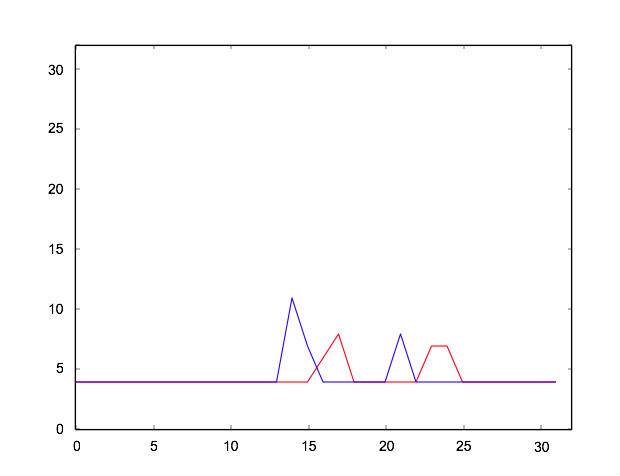
\includegraphics[height=60mm]{trees/gesture4-peaksize-smoothed2.jpg}
\caption{Geglätteter Graph anhand des am häufigsten vorkommenden Wertes}
\label{fig:frequent_value}
\end{figure}


Stark vereinfacht unterscheiden sich die Gesten dahingehend, ob und auf welcher Seite 
eine Veränderung der Anzahl aller zum Referenzton gehörenden Frequenzanteile stattfindet. 
Weiterhin muss unterschieden werden, in welche Richtung sich diese Verschiebung ausbreitet. 
Sie kann beispielsweise von der rechten zur linken oder von der linken zur rechten Seite 
um den Referenzton wandern, sowie gleichzeitig auf beiden Seiten stattfinden. 
Ein Beispiel dafür zeigt Abbildung~\ref{fig:left_right_same_time}

\begin{figure}[htbp] \centering
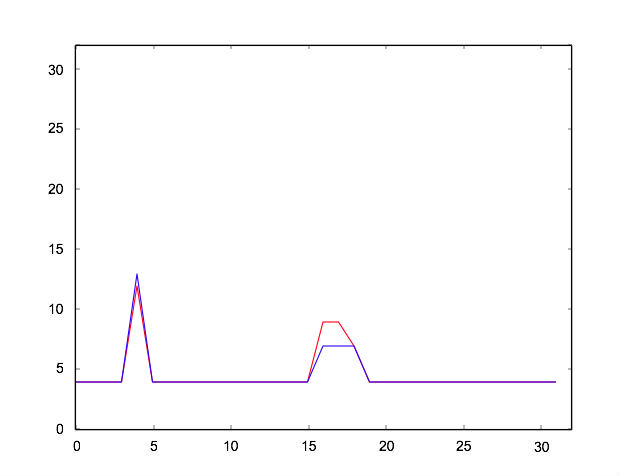
\includegraphics[height=60mm]{trees/gesture2-peaksize-smoothed2.jpg}
\caption{Gleichzeitige Verschiebung zur rechten und linken Seite des Referenztons}
\label{fig:left_right_same_time}
\end{figure}

Bei der in der Grafik abgebildeten Geste handelt es sich um ein mit der rechten und linken Hand entgegengesetztes zu und 
wegbewegen von dem Monitor, so dass gleichzeitig auf der rechten und linken Seite eine Vergrößerung der 
zum Referenzton gehörenden Frequenzanteile entsteht, was sich auch in der Grafik ablesen lässt.
%Diese Unterscheidungsmerkmale können sehr gut durch einen Entscheidungsbaum abgebildet werden. 
%Dazu kann die Verschiebungsrichtung als Maß dienen, um die Eingabemenge zu unterteilen und 
%somit eine Klassifizierung zu erreichen.

\subsection{Merkmalsextraktion}
Einleitungsblabla..

\subsubsection{Charakteristiken der Gesten} \label{charakteristiken}
Durch die Vorverarbeitung der Daten entstehen für die einzelnen Gesten Charakteristiken, anhand dessen sie unterschieden werden können. Nachfolgend wird zu sehen sein, dass sich einige der Gesten gut von den anderen abgrenzen lassen, andere sich dagegen stark ähneln.

\paragraph*{\acl{RLO}}
Die Geste \acl{RLO} beschreibt eine Bewegung mit der Hand von links nach rechts oder von rechts nach links, also bewegt sie sich zunächst auf den Sender zu und dann wieder von ihm weg. Dadurch entsteht zunächst eine Frequenzverschiebung auf der rechten Seite und danach auf der linken Seite des Frequenzspektrums. In Abbildung\ref{fig:left_right} wird eine typische Charakteristik mit der Verschiebung auf der rechten Seite (türkis) und auf der linken Seite (pink).

\begin{figure}[htbp] \centering
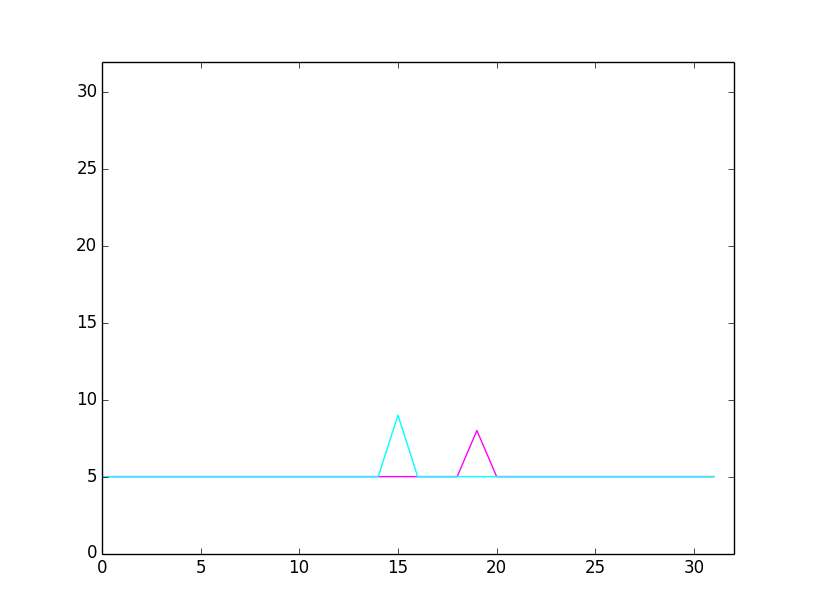
\includegraphics[height=60mm]{trees/left_right.png}
\caption{\acl{RLO}}
\label{fig:left_right}
\end{figure}


\paragraph*{\acl{TBO}}
In Abbildung~\ref{fig:top_bottom} ist die Geste \acl{TBO} abgebildet. Diese wird durch eine Bewegung mit der flachen Hand von oben nach unten ausgeführt. Dabei entsteht die Frequenzverschiebung auf der rechten Seite (türkis) und darauf folgend eine Frequenzverschiebung auf der linken Seite (pink). 

%\begin{figure}[htbp] \centering
%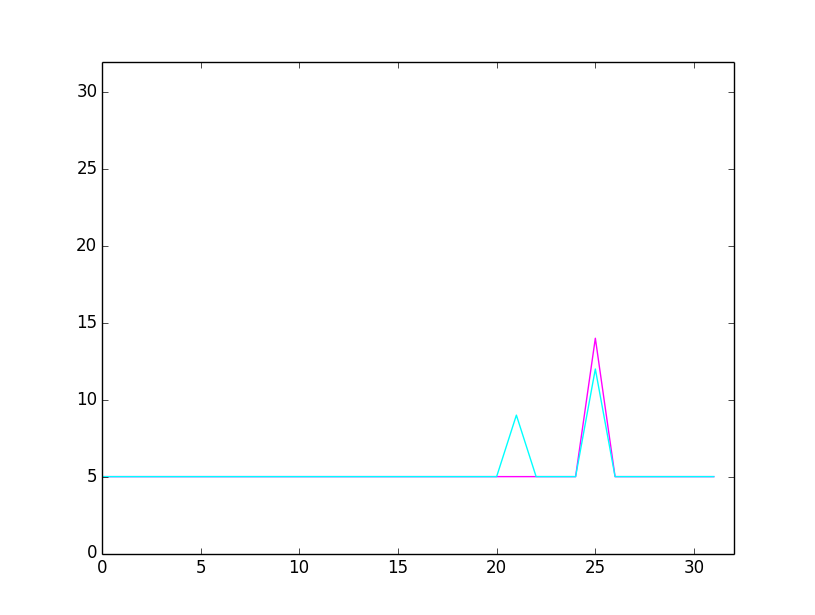
\includegraphics[height=60mm]{trees/top_bottom.png}
%\caption{\acl{TBO}}
%\label{fig:top_bottom}
%\end{figure}

\begin{figure}[htbp] \centering
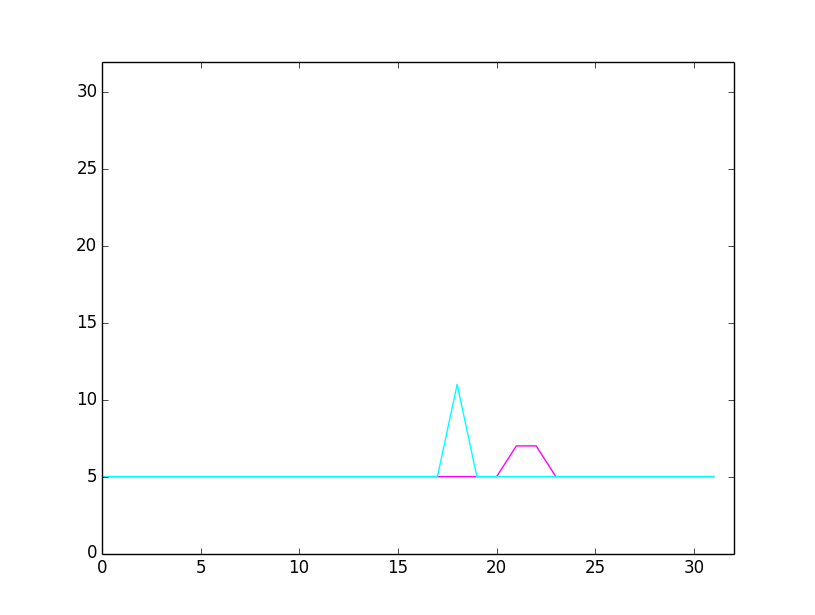
\includegraphics[height=60mm]{trees/top_bottom2.png}
\caption{\acl{TBO}}
\label{fig:top_bottom}
\end{figure}

\paragraph*{\acl{OT}}
Die in Abbildung~\ref{fig:contrary} dargestellten aufbereiteten Daten der Frequenzverschiebungen, die die Geste \glqq \acl{OT}\grqq\ erzeugt, zeigt üblicherweise je zwei gleichzeitige, also übereinander liegende, Frequenzverschiebungen. Dies ist dadurch zu erklären, dass zur selben Zeit eine Bewegung auf das Schallquelle zu und von dieser weg durchgeführt wird.

\begin{figure}[htbp] \centering
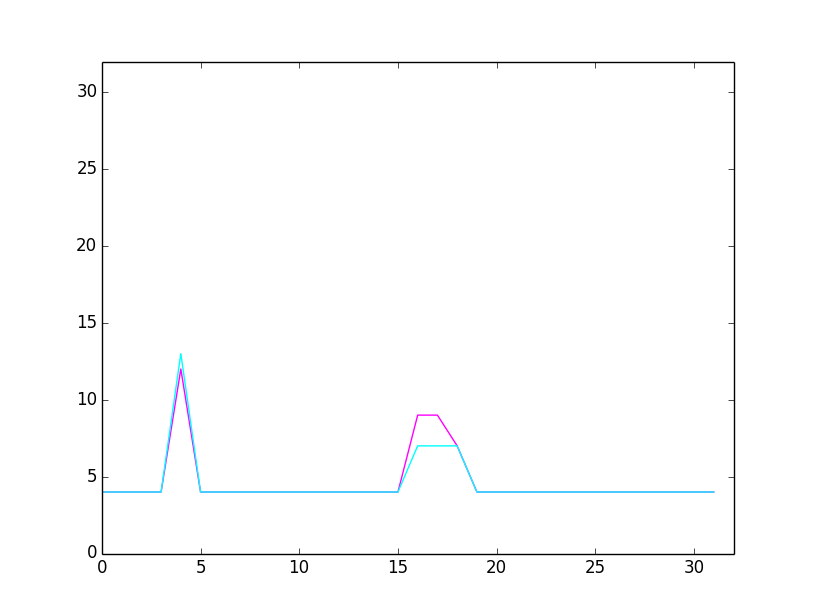
\includegraphics[height=60mm]{trees/contrary.png}
\caption{\acl{OT}}
\label{fig:contrary}
\end{figure}


\paragraph*{\acl{SPO}}
Der \glqq \acl{SPO}\grqq\ ist eine einfache Bewegung auf den Sender zu, sodass eine Frequenzverschiebung auf der rechten Seite des Frequenzspektrums festgestellt werden kann. Dies ist in Abbildung~\ref{fig:single_push} dargestellt.

\begin{figure}[htbp] \centering
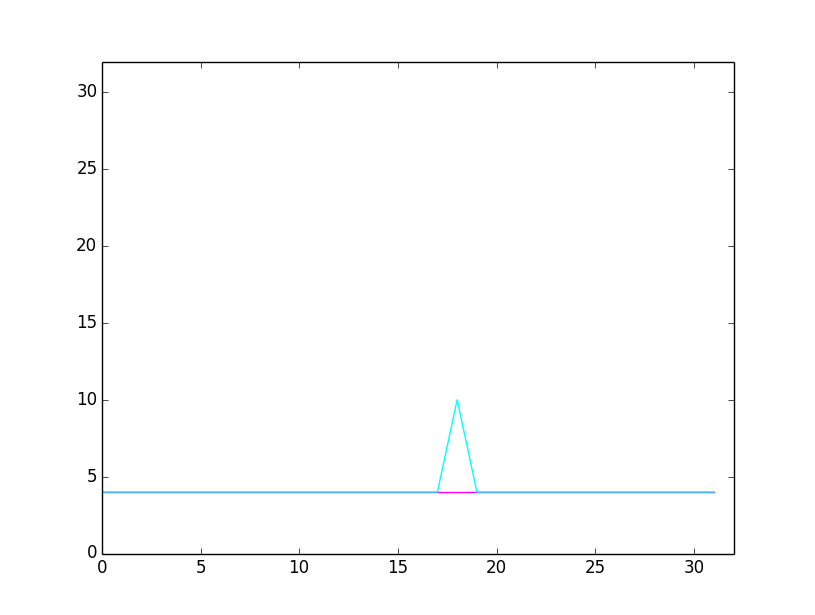
\includegraphics[height=60mm]{trees/single_push.png}
\caption{\acl{SPO}}
\label{fig:single_push}
\end{figure}

\paragraph*{\acl{DPO}}
Die charakteristischen Daten der Geste \glqq \acl{DPO}\grqq\ ist in Abbildung~\ref{fig:double_push} abgebildet. Sie zeichnet sich durch je zwei Verschiebungen auf der rechten und auf der linken Seite aus. Die Rechts-Links-Verschiebungen treten dabei kurz hintereinander auf und können sich auch teilweise überlappen. 

\begin{figure}[htbp] \centering
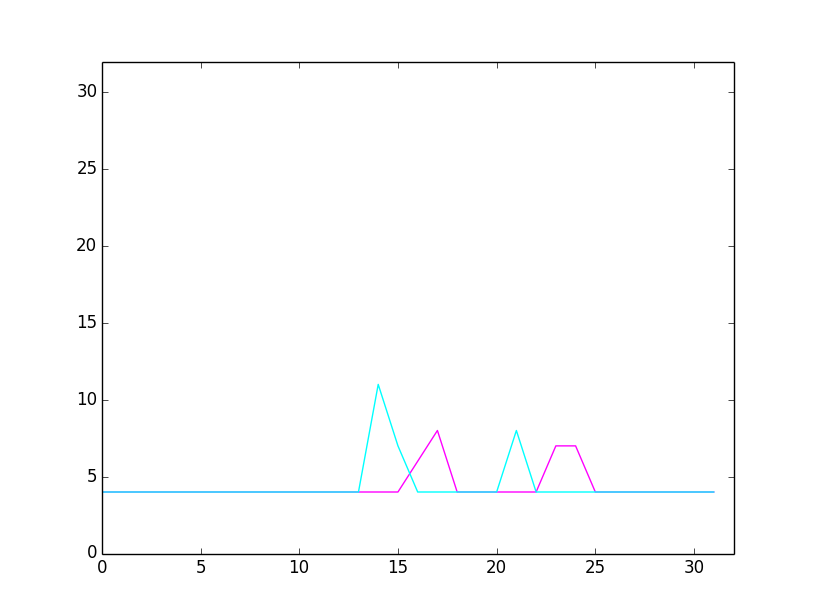
\includegraphics[height=60mm]{trees/double_push.png}
\caption{\acl{DPO}}
\label{fig:double_push}
\end{figure}

\paragraph*{Nothing}
Um später Gesten live zu erkennen, muss auch definiert sein, wann keine Geste auftritt. In diesem Fall ist in Abbildung~\ref{fig:nothing} keine Frequenzverschiebung zu erkennen. Der Graph zeigt keinen Ausschlag.

\begin{figure}[htbp] \centering
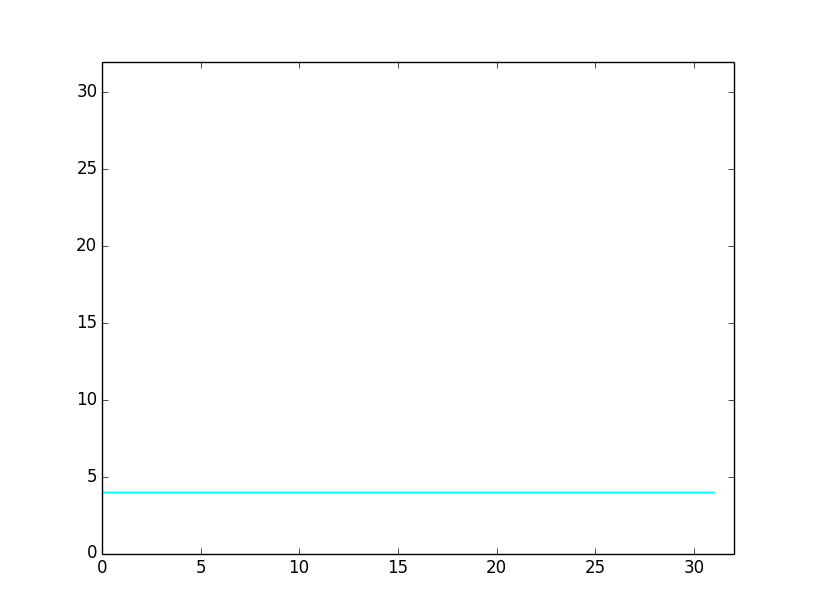
\includegraphics[height=60mm]{trees/nothing.png}
\caption{Keine Geste}
\label{fig:nothing}
\end{figure}

\subsubsection{??????}
Durch die Filterung und Glättung können nun die einzelnen Frequenzverschiebungen eindeutig identifiziert werden. Zudem ist in Abschnitt~\ref{charakteristiken} beschrieben, welche typische Gestalten der Graph für die verschiedenen Gesten annimmt. So lassen sich durch die Anordnung, Ausprägung und Aufkommen der Frequenzverschiebungen die unterschiedlichen Charakteristiken der einzelnen Gesten erkennen. Wie jedoch auch ersichtlich wurde, ähneln sich einige Gesten sehr stark, sodass eine Unterscheidung zum Teil auch mit bloßem Auge schwer fällt. Hier kommt die Merkmalsextraktion zum Tragen, denn sie soll unterstützen feine Unterschiede besser zu erkennen, indem sie stärker gewichtet werden. Das Ziel der Merkmalsextraktion ist es, aus den 32 Datenpunkten weitere eindeutige Merkmale herauszuarbeiten um schließlich einen Merkmalsvektor mit überschaubarer Anzahl an Merkmalen zu generieren. Um dies zu realisieren, wurden folgende Eigenschaften der einzelnen Gesten untersucht:

\begin{itemize} 
\item Anzahl der Frequenzverschiebungen
\item Zeitliche Abfolge der Frequenzverschiebungen
\item Anzahl der gleichzeitigen Frequenzverschiebungen
\item Amplitudenunterschiede zwischen den Frequenzverschiebungen
\end{itemize}

\paragraph*{Anzahl der Frequenzverschiebungen}
Die Anzahl der Frequenzverschiebung sagt bereits einiges über die Geste aus, wobei auch wichtig ist, ob die Frequenzverschiebungen im höheren oder niedrigeren Frequenzbereich liegen. Wie bereits in Abschnitt~\ref{sect:Trees_Datenaufbereitung} erwähnt, erzeugt eine Bewegung auf die Schallquelle zu eine Frequenzverschiebung auf der rechten Seite, also eine Ausdehnung in Richtung der höheren Frequenzen. Durch das Bewegen von der Schallquelle weg, erfolgt eine Frequenzverschiebung zur linken Seite, bzw. in Richtung der niedrigeren Frequenzen. 

Ein einfacher \glqq \acl{SPO}\grqq\ erzeugt deshalb im optimalen Fall eine Frequenzverschiebung auf der rechten Seite des Peaks. Wird die Hand wieder zurückgezogen, tritt auch eine Frequenzverschiebung auf der linken Seite auf. Klar davon abgegrenzt werden kann beispielsweise die Geste \glqq \acl{DPO}\grqq. Diese erzeugt mit dem Zurückziehen der Hand nach dem zweiten Push zwei Frequenzverschiebungen auf der linken und zwei auf der rechten Seite.

\paragraph*{Zeitliche Abfolge der Frequenzverschiebungen}
Ein weiteres Merkmal einer Geste ist die zeitliche Abfolge der Frequenzverschiebungen. Ein \glqq \acl{SPO}\grqq\ erzeugt zeitlich hintereinander erst eine Verschiebung rechts und dann eine Verschiebung links. Die in Abbildung~\ref{fig:contrary} dargestellte Geste \glqq \acl{OT}\grqq beschreibt dagegen die gleichzeitige gegensätzliche Bewegungen in Richtung der Schallquelle und von diesem weg. Somit tritt in diesem Fall gleichzeitig je eine Verschiebung nach rechts und links auf. 

\paragraph*{Anzahl der gleichzeitigen Frequenzverschiebungen}
Die beiden Gesten \glqq \acl{DPO}\grqq\ und \glqq \acl{OT}\grqq\ gehören zu den Gesten, die mehr Frequenzverschiebungen erzeugen als die häufige erst Rechts- dann Linksverschiebung. Dadurch sind sie sich ähnlich. Im optimalen Fall generiert Geste \glqq \acl{OT}\grqq\ gleichzeitige Frequenzverschiebungen auf beiden Seiten. Um die Anzahl der Falschklassifikationen zu verringern, werden die gleichzeitigen Frequenzverschiebungen gezählt und in den Merkmalsvektor aufgenommen. So wird die das Merkmal der Gleichzeitigkeit verstärkt.

\paragraph*{Amplitudenunterschiede zwischen den Frequenzverschiebungen}
Die Gesten \glqq \acl{SPO}\grqq\, \glqq \acl{TBO}\grqq\ und \glqq \acl{RLO}\grqq\ unterscheiden sich in der zeitlichen Abfolge der Verschiebungen nicht. In beiden Fällen tritt erst eine Verschiebung rechts, dann links auf. Jedoch unterscheiden sich die Verschiebungen an sich. Bei \glqq \acl{SPO}\grqq\ unterscheiden sich die beiden Verschiebungen im optimalen Fall nur dadurch, dass die eine Verschiebung links und die andere rechts vom Peak auftritt. Bei \glqq \acl{RLO}\grqq\ dagegen ist die Amplitude der zweiten Verschiebung, links vom Peak, schwächer als die andere.


\subsection{Implementierung}

Für die Datenaufbereitung und Merkmalsextraktion wurden in den Modulen GestureModel.py und Feature.py verschiedene Datentransformationen vorgenommen. Für die Klassifikation wurde auf Klassen und Methoden des Moduls \textit{sklearn.ensemble}~\cite{sklearn.ensemble} der Bibliothek \textit{sklearn}~\cite{sklearn} zurückgegriffen.

>> Datenaufbereitung
>> Merkmalsextraktion

Das Modul \textit{Feature.py} stellt einige Funktionen zur Merkmalsextraktion bereit. In Abschnitt~\ref{subsec:featureextraction} sind die erkennbaren Charakteristiken der einzelnen Gesten beschrieben und auch das Problem der Ähnlichkeit einiger Charakteristiken beschrieben. 

\subsection{Evaluation}

\subsection{Fazit}

